\frame{
  \frametitle{Tutte}
\framesubtitle{Tutte's theorem}    
  \begin{figure}[H]
    \centering
    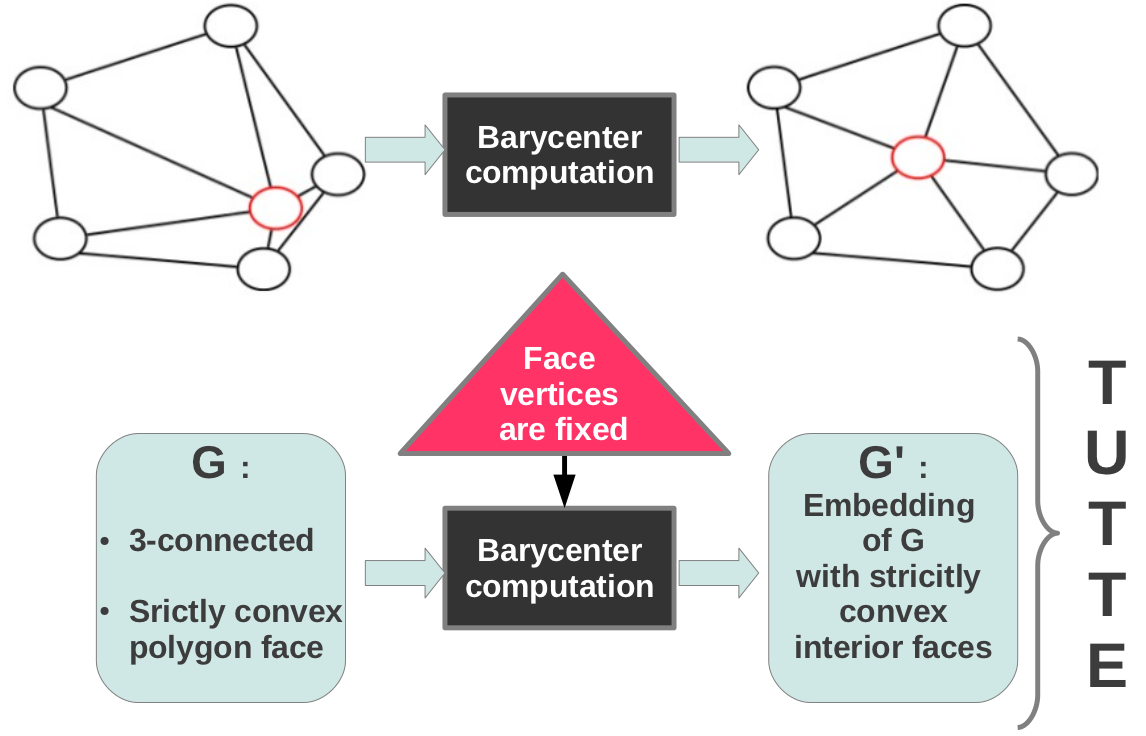
\includegraphics[scale=0.29]{../rapport/img/tutte.png}
  \end{figure}
} 

\frame{
  \frametitle{Tutte}
  \framesubtitle{Tutte's theorem and polygone concave face}
\begin{figure}[H]
    \centering
    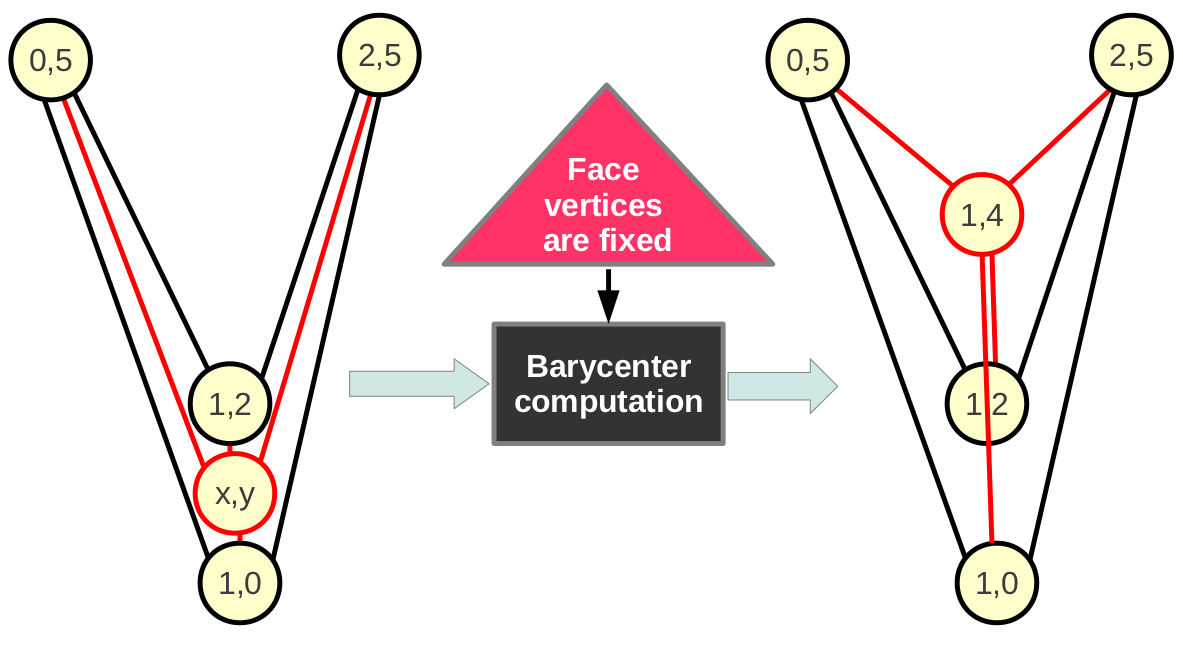
\includegraphics[scale=0.29]{../rapport/img/tutte2.png}
  \end{figure}
} 

\frame{
  \frametitle{Tutte}
\framesubtitle{Tutte's theorem and fixed vertices}
\begin{figure}[H]
    \centering
    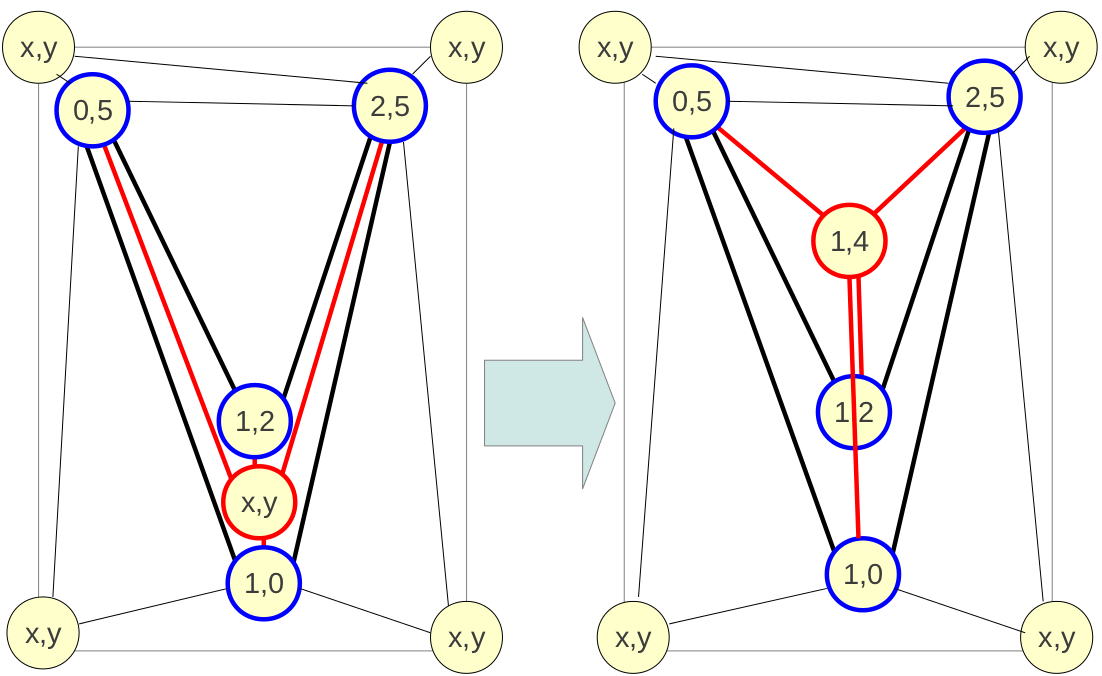
\includegraphics[scale=0.29]{../rapport/img/tutte3.png}
  \end{figure}


} 
